\section{The Team}
The team consists of seven students from NTNU. About half of the members have worked
together on previous projects and therefore have experience functioning together as a
team. Having a properly functioning team where all the skills of each team member is properly
utilized is vital for the success of any project. None of the team members have any experience 
working for a customer so we have to prepare for any challenges this might cause.


\subsection{Project Roles}
Roles of each member? Scrum Master, Team Leader, Customer Relations, etc.

\subsection{Anders Eie}
???

\subsection{Jonas Svarvaa}
Third year student at NTNU. Experience with Java, Python, Lua, PHP, and web standards such as HTML, CSS and Javascript. Previously worked with media and sound engineering.

\subsection{Johan Jansen} 
Third year student at NTNU. Experience with the programming languages Java, C, C++  and 
Basic. Worked with AVR microcontrollers in other projects and courses.

\subsection{Asbjørn Lucassen}
???

\subsection{Emanuel Di-Santo}
???

\subsection{Bjørnar Wold}
???

\subsection{Henrik Goldsack}
???

\newpage
\section{Selecting Development Process}
Choosing a development process is crucial for every project as many varying factors such as
project size, members and time affect which process is suitable. The following section describes
which development processes we have considered using. The choice of the development method
will affect how the group communicates, collaborates and write the code.

\subsection{Waterfall}
The Waterfall model is a strict top-down design process. It features detailed planning, design and
documentation before design. The strict model is useful where going back and changing requirements is 
costly or impossible. This does however require that all needed features and requirements are known
early on. The model was originally used for hardware design and when the first software projects 
appeared it was simply adapted. Many argue that the Waterfall model is bad for software design, seeing
as the developers cannot predict all problems or additional requirements before reviewing a working
prototype of the final product. Customers also often have changing requirements under development.
The Waterfall model works best for expensive projects where problem prediction and initial correct design
is vital before implementation is started.
\begin{figure}[h!]
\centering 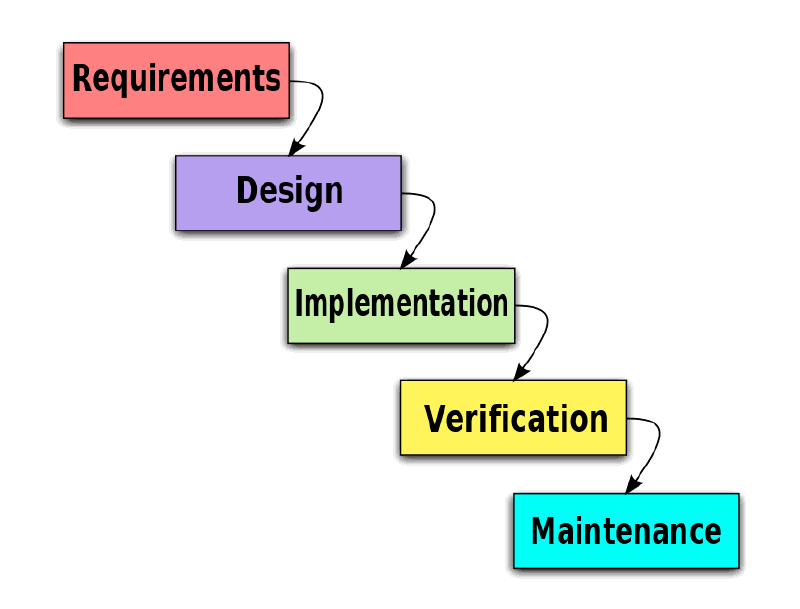
\includegraphics[scale=0.30]{img/designmodel-waterwall} \caption{The Waterfall model}
\label{fig:desigmodel-waterfall}
\end{figure}

\subsection{Scrum}
Scrum is a for of agile project managment. The scrum approach uses  repetitive iterations (called 
a Sprint in the Scrum etymology) to design, implement and refine a product. Each iteration improves,
fixes and adds new features to the previous iteration. A key feature of Scrum is that the customer
can change their mind on what they want or need. Scrum focuses on frequent group meetings and
splitting big tasks into lesser, managble tasks for smaller groups of programmers. Because of the
frequent meetings it promotes verbal communication in the group.
\begin{figure}[h!]
\centering 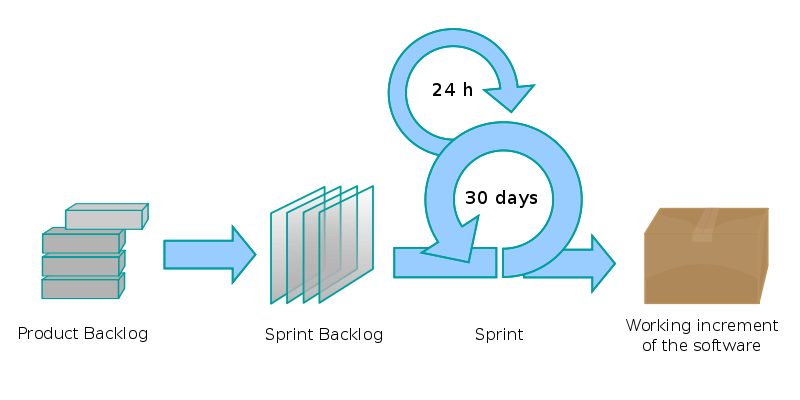
\includegraphics[scale=0.4]{img/designmodel-scrum} \caption{The Scrum process}
\label{fig:desigmodel-scrum}
\end{figure}

\subsection{Extreme Programming (XP)}
Extreme Programming is a development methodology that is designed for best software quality and
quick responsivness to changing customer requirements. It is also an Agile Development method like
Scrum and therefore shares certain similarities to that development method. It promotes rapid
development and allows the customer to change his/her mind or request new features throughout
the development of the software. Typical elements for XP are pair programming, unit testing,
lazy programming, simplicity and expecting changes in customer requirements as time passes
and the problem is better understood. Several pitfalls include buggy and unstable code or lack of
overall design specification. Extreme programming is best suited for small projects for prototyping
where the customer is not entierly sure what he or she wants.
\begin{figure}[h!]
\centering 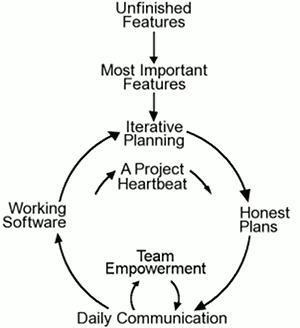
\includegraphics[scale=0.75]{img/designmodel-xp} \caption{Extreme Programming}
\label{fig:desigmodel-xp}
\end{figure}

\subsection{Agile Unified Process}
The AUP (short for Agile Unified Process) offers a simple and easy to understand approach for software
development. It is a simplified version of the Rational Unified Process. Key features are simplicity, 
customization and focus on the task on hand instead of everything that may or will happen. It features 
several internal development iterations before producing a customer release. AUP focuses on quality
insurance and works best for projects that is going to be used by a large public and a working, bugfree
product is important.
\begin{figure}[h!]
\centering 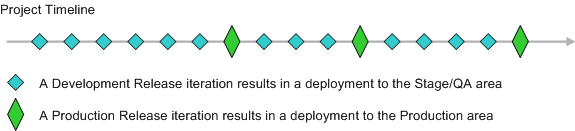
\includegraphics[scale=0.65]{img/designmodel-aup} \caption{AUP development iterations}
\label{fig:desigmodel-aupl}
\end{figure}

\subsection{Spiral Model}
The Spiral development methodology combines the advantages of both the top-down approach from 
Waterfall and the bottom-up concept of prototyping. It does this by using iterative development and
controlling it through the systematic Waterfall model. A strong advantage of the Spiral lifecycle is that it
allows new features and requests to be integrated as soon as they come avalible or known. Other key 
features of the model is risk analysis, strict sysem design specifications and prototyping. The Spiral model
 is best suited for large, expensive and complicated projects.
\begin{figure}[h!]
\centering 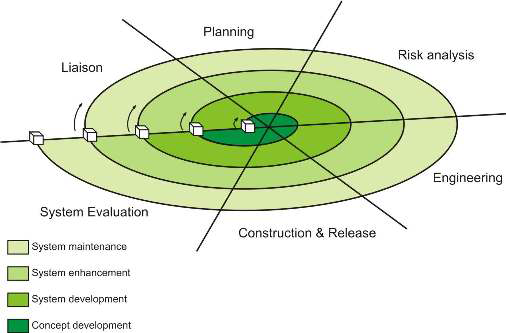
\includegraphics[scale=0.85]{img/designmodel-spiral} \caption{The Spiral model}
\label{fig:desigmodel-spiral}
\end{figure}

\subsection{Conclusion}
We initially selected Scrum as our development process. The arguments  for using Scrum were that we would
have a work schedule that fit into a iterative process in addition to weekly meetings with a customer that
wanted a new version of the prototype each sprint. Moreover everyone in the team had existing experience 
with Scrum from previous projects. After a few weeks of development however, we observed that the Scrum
model did not fit our project. Unspecific and unclear requirements from the customer lead along with
the customer wanting a working prototype from week 1 meant we had to change our entire development
process. This cost us a lot of work since we had already setup and planned the project using Scrum 
development methodology, but after each meeting of the customer the entire project goal changed. This
lead us into researching using either Extreme Programming or the Spiral model. After the third week we
adapted the Extreme Programming process.

%TODO: explain why we selected XP!

\section{Project management tools}

%this part needs to be rewritten!
\textcolor{red}
{
To accompany us in the Scrum process we have chosen an online tool
called ScrumDo (www.scrumdo.com). This tool has features for most
if not all parts of the Scrum process. Using this tool consistently
will be our main method of maintaining and separating packages from
the WBS (Work Breakdown Structure). In the context of ScrumDo and
Scrum these low level work packages are called stories and are moved
accordingly from \char`\"{}ToDo\char`\"{} over to \char`\"{}In progress\char`\"{}
and eventually to \char`\"{}Done'' areas.
}
	
\begin{figure}[h!]
\centering 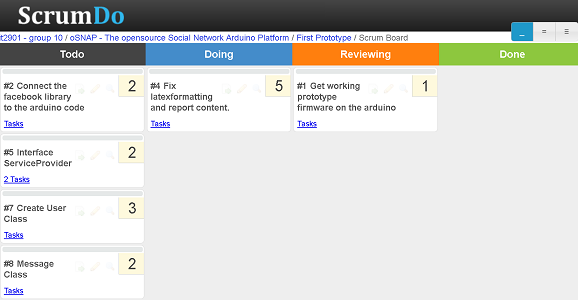
\includegraphics{img/management-scrumdo} \caption{The Scrum Board in ScrumDo}

\label{fig:management-scrumdo}
\end{figure}
	
Another part of the project is the collaboration software.
Initially we decided to use Git which is a fast, scalable,
distributed revision control system with an unusually rich command
set that provides both high-level operations and full access to internals.
It differs from the centralised control systems like SVN for its capability
to handle several software \char`\"{}branches\char`\"{} at once. The
branches can head in different directions and can later be merged
instead of always maintaing a central, \char`\"{}correct\char`\"{}
version. NTNU provided SVN and Trac repositories to keep track of our
project and we will use these to share finished code for evaluation
purposes. We decided to use Git due to its higher flexibility and because
of the experiences the team members already had with it.

\newpage
\section{Risk analysis and mitigation strategies}

This text will highlight different realistic risks that may occur during development
that can to some degree jeopardise the process or the final product.
A table with weighted risks and relative mitigation and remedial actions follows.

\begin{itemize}
\item Dropouts
\end{itemize}
The risk of people dropping the course or otherwise not being able to complete it as part
of the group. This can be caused by sickness as well.

\begin{itemize}
\item Arduino hardware
\end{itemize}
Our handed out Arduino equipment can fail, due to malfunctioning or wrong usage.
There is also the possibility that some of the hardware can be lost while we work with it at home.

\begin{itemize}
\item Deadlines
\end{itemize}
Throughout the course there is multiple deadlines that must be met. Failure to meet
these limits will have huge impacts on the grading and could possibly fail the group.

\begin{itemize}
\item Choosing wrong frameworks
\end{itemize}
We will necessarily have to build parts of our software around existing open source
frameworks to limit effort required by the task. If at a later point we have severe limitations
on our possibilities due to these frameworks the product could result poorer in features than
we originally planned. The impact can be negligible if other solutions are found.

\begin{itemize}
\item Design problems
\end{itemize}
During development features have to be constrained due to problems or resource limitations.
This will in turn will cause the final product to not satisfy the customer. If we can find work-arounds
and compromises can be found, then the problem will not have as huge of an impact.

\begin{itemize}
\item Wireless connectivity
\end{itemize}
If the Arduino chip modules (called shields) for Bluetooth etc. are too hard to implement
we would have to reconsider wireless connectivity as an option.
We set the 'get wireless to work' deadline to be one month. If we can't get it working
by that time we will have to use cabled connections instead and that would result clumsy
for a lot of concepts.

\begin{table}
	\begin{center}
		\begin{tabular}{| l | l | l | l | p{2.8cm} | p{2.8cm} |}
\hline

Description & Likelihood & Impact & Risk & Mitigation & Remidial Action\\ \hline

Sickness 			& Med & Low & Med & Keep contagious sicknesses at home.
					& If the sickness is prolonged work tasks must be re-arranged appropriately. \\

Wireless Connect. & Low & High & Med & Get it working & Switch to cable connection \\

Arduino Malfun. & Low & Med & Low & Treat hardware properly. Do not eat or drink nearby.
					&  Get new hardware if possible.\\

Lost Hardware & Low & Med & Low & Have control over who has what and keep an inventory list.
					& Get new hardware if possible \\

Limited Product & Low & Med & Low & Thorough planning. Avoid late features implementation.
					&  Workaround problems at critical junctions in the process.\\

API Trouble & Med & Med & High & Limit the scope to documented open source APIs.
			& Investigate alternative solutions. Limit impact on productivity. \\

Final Deadline & Low & High & Med & Consistent work throughout the semester. Avoid last-minute feature implementation.
			&  Deliver the product in the best state possible.\\
Mid-Sem Deadline & Low & High & Med & Produce good documentation and begin early on reports.
			&  Consult with student assistants.\\
		\hline
		\end{tabular}
	\end{center}
	\caption{Risk Analysis}
	\label{table:riskanalysis}
\end{table}

Concluding, most care should be put in the choice of existing frameworks and in early planning
and documentation efforts to avoid later problems related to the implementation and report delivery.

